
\documentclass[calculator,allquestions,datasheet,solutions]{exam_newMarcus2}
%\documentclass[calculator,allquestions,datasheet]{exam_newMarcus2}

% The full list of class options are
% calculator : Allows approved calculator use.
% datasheet : Adds a note that data sheet are attached to the exam.
% handbook : Allows the use of the engineering handbook.
% resit : Adds the resit markings to the paper.
% sample : Adds conspicuous SAMPLE markings to the paper
% solutions : Uses the contents of \solution commands (and \solmarks) to generate a solution file

\usepackage{pdfpages}  
\usepackage{lscape,comment} 
 
\coursecode{EX3029}%% 
\coursetitle{Chemical Thermodynamics}
 
\examtime{00.00--00.00}%
\examdate{15}{12}{2017}% 
\examformat{Candidates must attempt \textit{all} questions, each of which carries equal (20) marks.  All thermodynamic symbols have their usual meanings unless otherwise stated.}

% Other symbols
\newcommand{\frc}{\displaystyle\frac}
\newcommand{\br}[1]{\!\left( #1 \right)}
\newcommand{\abs}[1]{\left| #1 \right|}
\newcommand{\fracd}[2]{\frac{\mathrm{d} #1}{\mathrm{d} #2}}
\newcommand{\fracp}[2]{\frac{\partial #1}{\partial #2}}
\renewcommand{\d}[1]{\mathrm{d} #1 } 
\newcommand{\Ma}{\mathrm{M\!a}} 
\newcommand{\eg}{{\it e.g., }}
\newcommand{\ie}{{\it i.e., }}
\newcommand{\wrt}{{\it wrt }}
\newcommand{\Partial}[3][error]{\left(\frc{\partial #1}{\partial #2}\right)_{#3}}
\newcommand{\mfr}[3][error]{#1_{#2}^{\left(#3\right)}} 
\newcommand{\summation}[3][error]{\sum\limits_{#2}^{#3}#1}


\begin{document}


%%%
%%% Question 01 
%%%
\begin{question}
  \begin{enumerate}[a)]
     \item Using the definitions
        \begin{displaymath}
           \alpha = \frc{1}{V}\left(\frc{\partial V}{\partial T}\right)_{P}, \hspace{1cm} \beta = -\frc{1}{V}\left(\frc{\partial V}{\partial P}\right)_{T}\hspace{1cm}\text{ and }\hspace{1cm}  \left(\frc{\partial P}{\partial T}\right)_{V}\left(\frc{\partial V}{\partial P}\right)_{T}\left(\frc{\partial T}{\partial V}\right)_{P} = -1,
        \end{displaymath}
        show that 
        \begin{displaymath}
          \left(\frc{\partial P}{\partial T}\right)_{V} = \frc{\alpha}{\beta}
        \end{displaymath}\marks{8}
%====================
        \solution{ From the cyclic rule applied to $PVT$ relations,
           \begin{displaymath}
              \left(\frc{\partial P}{\partial T}\right)_{V}\left(\frc{\partial V}{\partial P}\right)_{T}\left(\frc{\partial T}{\partial V}\right)_{P} = -1.
           \end{displaymath}
           Thus,\solmarks{8}
           \begin{displaymath}
             \left(\frc{\partial P}{\partial T}\right)_{V} = \frc{-1}{\left(\frc{\partial V}{\partial P}\right)_{T}\left(\frc{\partial T}{\partial V}\right)_{P}} = \frc{-\left(\frc{\partial V}{\partial T}\right)_{P}}{\left(\frc{\partial V}{\partial P}\right)_{T}} = \frc{-V\alpha}{-V\beta} = \frc{\alpha}{\beta}
           \end{displaymath}
        }
%====================================================
%%% Moran & Shapiro (Example 11.5)      
     \item Using the Redlich - Kwong equation of state, develop algebraic expressions for the changes in specific entropy and internal energy of a gas between two states where the temperature is the same, $T_{1}=T_{2}$, and the pressures are $P_{1}$ and $P_{2}$, respectively.\marks{12}
%====================
        \solution{The RK EOS is explicit in pressure,
           \begin{displaymath}
             P = \frc{R T}{v-b} - \frc{a}{v\sqrt{T}\left(v+b\right)},
           \end{displaymath}
           and in order to obtain $u_{2}-u_{1}$, $s_{2}-s_{1}$ we should integrate
           \begin{displaymath}
             \begin{cases}
               ds = \frc{C_{v}}{T}dT + \Partial[P]{T}{v}dv & \\
               du = C_{v}dT + \left[T\Partial[P]{T}{v}-P\right]dv & \\
             \end{cases}
           \end{displaymath}
          At the isotherm $T_{1}=T_{2}$,\solmarks{2/12}
           \begin{displaymath}
             \begin{cases}
               s_{2}-s_{1} = \displaystyle\int\limits_{v_{1}}^{v_{2}} \Partial[P]{T}{v}dv, & \\
               u_{2}-u_{1} = \displaystyle\int\limits_{v_{1}}^{v_{2}} \left[T\Partial[P]{T}{v}-P\right]dv. & \\
             \end{cases}
           \end{displaymath}
           The limits for the integrals are the specific volumes $v_{1}$ and $v_{2}$ at the two states under consideration. Using $P_{1}$ and $P_{2}$ and the known temperature, $T_{1}=T_{2}=T$, these specific volumes should be readily obtained from the RK EOS. Before integrating, we need to solve the partial differential $\Partial[P]{T}{v}$ for the RK EOS,\solmarks{2/12}
           \begin{displaymath}
             \Partial[P]{T}{v} = \frc{R}{v-b} + \frc{a}{2v\left(v+b\right)T^{3/2}}.
           \end{displaymath}
           Now solving for the change in entropy,\solmarks{3/12}
           \begin{eqnarray}
             s_{2}-s_{1} &=& \displaystyle\int\limits_{v_{1}}^{v_{2}} \left[\frc{R}{v-b} + \frc{a}{2v\left(v+b\right)T^{3/2}}\right]dv \nonumber \\
                        &=& R \ln{\left(\frc{v_{2}-b}{v_{1}-b}\right)} + \frc{a}{2bT^{3/2}}\left[\ln{\frc{v_{2}}{v_{1}}}-\ln{\frc{v_{2}+b}{v_{1}+b}}\right] \nonumber \\
                        &=& R \ln{\left(\frc{v_{2}-b}{v_{1}-b}\right)} + \frc{a}{2bT^{3/2}}\ln{\frc{v_{2}\left(v_{1}+b\right)}{v_{1}\left(v_{2}+b\right)}}.\nonumber
           \end{eqnarray}
           For the change in internal energy, the term in bracket\solmarks{2/12}
           \begin{displaymath}
             \left[T\Partial[P]{T}{v}-P\right] = \frc{3a}{2v\left(v+b\right)T^{1/2}},
           \end{displaymath}
           need to be integrated from $v_{1}$ to $v_{2}$,\solmarks{3/12}
           \begin{eqnarray}
             u_{2}-u_{1} &=& \displaystyle\int\limits_{v_{1}}^{v_{2}} \frc{3a}{2v\left(v+b\right)T^{1/2}}dv \nonumber \\
                        &=& \frc{3a}{2bT^{1/2}}\left[\ln{\frc{v_{2}}{v_{1}}} - \ln{\frc{v_{2}+b}{v_{1}+b}}\right] \nonumber \\
                        &=& \frc{3a}{2bT^{1/2}}\left[\ln{\frc{v_{2}\left(v_{1}+b\right)}{v_{1}\left(v_{2}+b\right)}}\right].\nonumber
           \end{eqnarray}
        }
%====================================================
  \end{enumerate}
  
  
\end{question}

\clearpage


%%%
%%% Question 02
%%%
\begin{question}
\end{question}

\clearpage



%%%
%%% Question 03
%%%
\begin{question}
\end{question}

\clearpage


%%%
%%% Question 04
%%%
\begin{question}
\end{question}

\clearpage

%%%
%%% QUESTION 05
%%%
\begin{question}
\end{question}


\vfill
\paperend



\vfill 



%\begin{comment}
{
  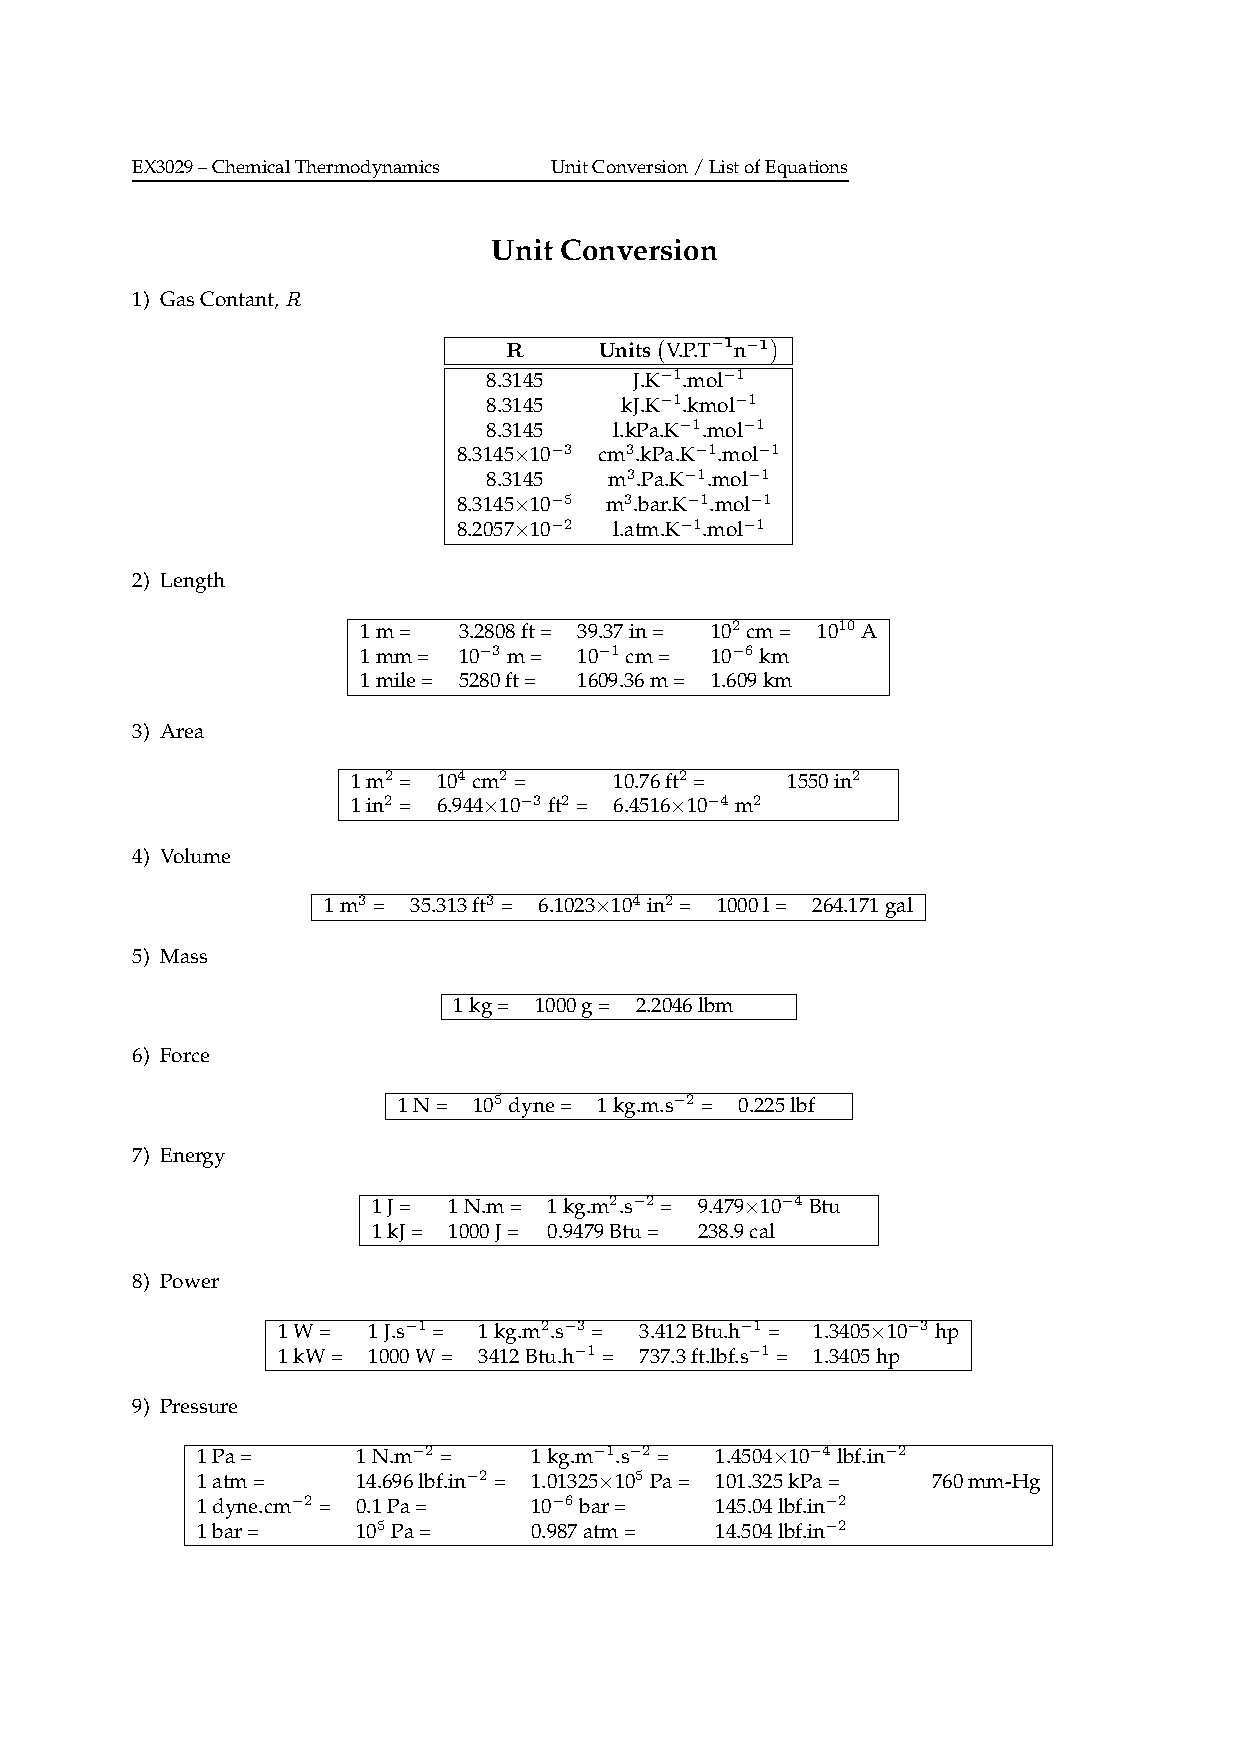
\includepdf[pages=-,fitpaper]{./Pics/EquationsList}
}
%\end{comment}



\end{document}
